\documentclass{article}

\usepackage{geometry}
\geometry{
	a4paper,
	total={170mm,257mm},
	left=20mm,
	top=20mm,
}

\usepackage{amsmath}
\usepackage{amsfonts}
\usepackage{amsthm}
\usepackage{graphics}
\usepackage{graphicx}

%\setlength{\parskip}{6pt}

\newtheorem{property}{\hskip3\labelsep Property}
\newtheorem{lemma}{\hskip3\labelsep Lemma}
\newtheorem{statement}{Statement}

%\usepackage{xpatch}
%\xpatchcmd{\proof}{\hskip\labelsep}{\hskip4\labelsep}{}{}
%\makeatletter



\title{Self Driving Car Racing: Application of Deep Reinforcement Learning}
\author{}

\begin{document}
\section{Introduction}
\subsection{Motivation}
Car racing provides a unique and controlled environment for testing and advancing critical aspects of autonomous driving. While the objectives of racing and traditional road driving differ, the challenges inherent in racing align closely with key requirements for autonomous driving systems, such as real-time decision-making, handling dynamic environments, and optimizing complex behaviors under uncertainty. Tackling car racing tasks using Deep Reinforcement Learning (DRL) offers valuable insights and advancements that can be applied to broader autonomous driving applications.

Exploration is a cornerstone of reinforcement learning, particularly in car racing environments where:

Sparse and Delayed Rewards: Rewards, such as completing laps quickly or avoiding crashes, are often sparse and delayed, making it challenging to guide the agent effectively toward optimal policies.
Complex State and Action Spaces: Racing tasks involve continuous control over acceleration, steering, and braking in a high-dimensional state space. Insufficient exploration can result in agents getting stuck in suboptimal behaviors, such as driving in circles or failing to navigate challenging corners.

\subsection{Novelty}
Designing an appropriate reward function for a car racing task can be non-trivial. Unlike traditional programming approaches, reinforcement learning shifts the focus from explicitly encoding specific behaviors to designing reward systems that enable agents to autonomously discover optimal policies. This highlights the need for improved exploration strategies to ensure that agents explore different trajectories, learn robust behaviors, and avoid premature convergence to suboptimal solutions.

In this project, we systematically evaluate and compare different exploration strategies, including noise network \cite{NoisyNet}, dropout the policy layer \cite{DP}, ICM \cite{ICM} and RE3 \cite{RE3}, by leveraging A2C as a baseline. We gain insights into their impact on agent performance and highlight the broader applicability of DRL in advancing autonomous driving systems. Furthermore, we investigate the performance of traditional controllers MPC and PID in car racing and compare with our RL-based results. Further work is conducted on imitation learning.

\section{Preliminary}
\subsection{A2C}
A2C is a synchronous version of the Actor-Critic method. All workers or environments synchronize their gradients and parameters before performing updates. Stability in training due to synchronized updates across multiple environments.
\textit{Actor} is updated using the policy gradient:
\begin{align*}
\nabla_{\theta}J=\mathbb{E}[\nabla_\theta log\pi_\theta(a|s)A(s,a)].
\end{align*}
\textit{Critic} minimizes the temporal-difference (TD) error to learn the value function:
\begin{align*}
L(\phi) = \mathbb{E}[(r+\gamma V_{\phi}(s')-V_{\phi}(s))^2].
\end{align*}
Compute the advantage $A(s,a)$ using either:
\begin{align*}
A(s,a) &= r+\gamma V(s') -V(s)\ \ (1-step),\\
A(s,a) &= \sum_{t=0}^T \gamma^t r_t -V(s)\ \ (n-step).
\end{align*}
Since we have multi process, Aggregate gradients from all workers and update the model.
\subsection{Noise Network}
NoisyNets are a class of neural networks in which weights and biases are perturbed by noise scaled by learnable parameters. These parameters are optimized through gradient descent. In the Advantage Actor-Critic (A2C) algorithm, the architecture typically includes a final fully connected layer with an input dimension matching the size of the embedding vector and an output dimension of one to approximate the value function. Additionally, another fully connected layer is used to generate actions, with the input dimension matching the embedding vector and the output dimension equal to the size of the action space.

Building on the concept of noisy networks, the authors modify the final layer as follows:
\[
y = wx+b
\]
to 
\[
y = (\mu^w+\sigma^w\odot \epsilon^w)x+(\mu^b+\sigma^b\odot \epsilon^b),
\]
where $\mu^w+\sigma^w\odot \epsilon^w$ and $\mu^b+\sigma^b\odot \epsilon^b$ replace $w$ and $b$, respectively. The parameters $\mu^w$,$\mu^b$,$\sigma^w$,$\sigma^b$ are learnable whereas $\epsilon^w$ and $\epsilon^b$ are noise random variables.

\begin{figure} [!ht]
	\centering
	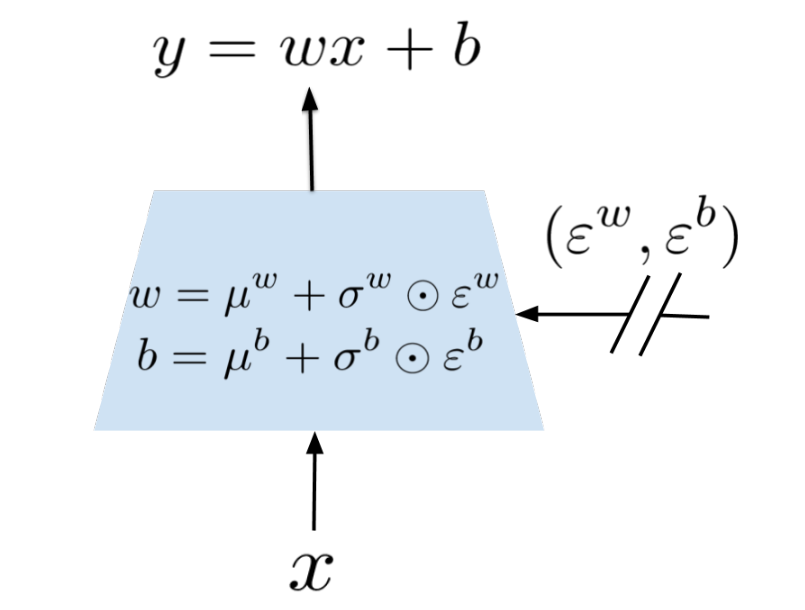
\includegraphics[width=0.35\linewidth]{figure/NoiseNet.png}
	\caption{Graphical representation of a noisy linear layer. The parameters $\mu_w$ , $\mu_b$ , $\sigma_w$ and $\sigma_b$ are the learnables of the network whereas $\epsilon_w$ and $\epsilon_b$ are noise variables. The noisy layer functions similarly to the standard fully connected linear layer.}
	\label{fig:enter-label}
\end{figure}
\subsection{Random Encoders for Efficient Exploration}
Analyzing real-world cases with continuous action and state spaces, we face the challenge that each state-action pair appears only once in the training set. The probability of observing the same state again in the future is nearly "zero." Therefore, it is essential to search for methods that group similar states and actions efficiently. The primary goal of the Random Encoder for Efficient Exploration (RE3) method is to minimize the number of training samples required for the model.

Convolutional networks are capable of identifying both external characteristics and internal features of individual objects. Even when convolutional encoders are initialized with random parameters, they can effectively capture information about the similarity between two states. The authors of the RE3 method propose maximizing the state entropy estimate within a fixed representation space of a randomly initialized encoder during model training. The main idea of RE3 is to estimate entropy using a k-nearest neighbors (k-NN) estimator in the low-dimensional space obtained by the randomly initialized encoder. The authors suggest calculating the distances between states in the representation space $f(\theta)$ of the random encoder, where the $\theta$ parameters are randomly initialized and fixed throughout the training process.

The intrinsic reward is represented as:
\begin{align*}
	r^i(s_i) = \log\left(\left\Vert y_i-y_i^{k-NN}\right\Vert_2+1\right),
\end{align*}
where $y_i$ is the state representation in then random encoder space.


\subsection{Intrinsic Curiosity Method}
Making predictions directly in the raw sensory space is suboptimal, as it is not only computationally challenging to predict pixel values accurately, but also unclear whether pixel prediction aligns with the objectives of the underlying task. Instead, this method focuses on computing curiosity within a latent space, where features are more abstract and meaningful. To achieve this, the approach introduces three neural network components: a state encoder, a forward model, and an inverse model. These components collectively enable the agent to process and interpret latent representations, facilitating more effective learning and exploration.
\begin{figure}
	\centering
	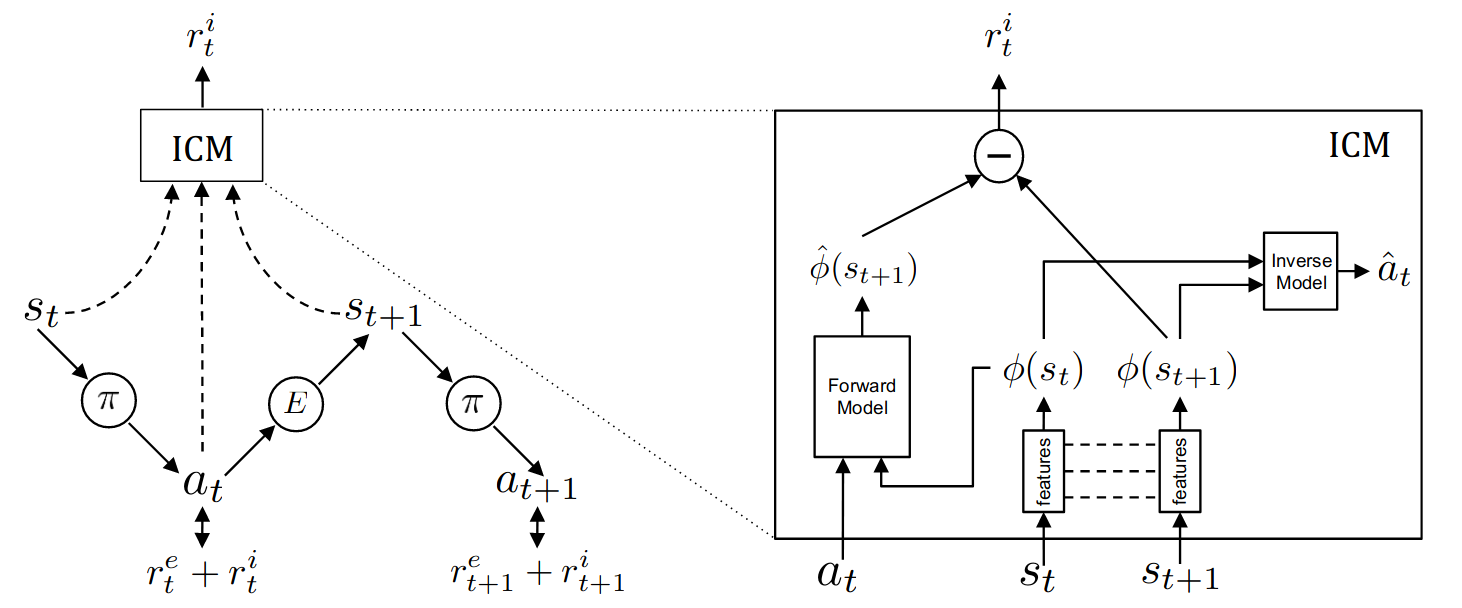
\includegraphics[width=0.5\linewidth]{figure/ICM_structure.png}
	\caption{The structure of ICM}
	\label{fig:enter-label}
\end{figure}
Assume we have the state $s_t$, $s_{t+1}$ and $a_t$ reprsent the observation at time $t$, the observation at time $t+1$ and the action applied to agent at time $t$.
The first sub-module encodes the raw state $s_t$ in to a feature vector $\phi(s_t)$. The second sub-module or so-called inverse model takes the feacture vectors $\phi(s_{t+1})$ and $\phi(s_t)$ as inputs to predict the action $a_t$:
\[
\hat{a}_t=g\left(s_t,s_{t+1};\theta_I \right).
\]
The loss function is $\min_{\theta_I}L_I(\hat{a}_t,a_t)$.

In addition to inverse dynamics model, this method also train another neural network (forward dynamics model) that takes as inputs $a_t$ and $\phi(s_t)$ and predicts the feature encoding of the state at time step $t+1$
\[
\hat{\phi}(s_{t+1}) = f\left(\phi(s_t),a_t;\theta_F\right).
\]
The loss function is $\frac{1}{2}\Vert \hat{\phi}(s_{t+1})-\phi(s_{t+1})\Vert^2$.

The intrinsic reward signal $r_t^i$ is computed as 
\[
r_t^i = \frac{\eta}{2}\Vert\hat{\phi}(s_{t+1}-\phi(s_{t+1})\Vert^2,
\] where $\eta>0$ is a scaling factor.
Here is the back propagation of the ICM. The prediction error of the forward model is only used to train the forward model, not the encoder. The inverse prediction error of the inverse model is used to train both the inverse model and the encoder. The prediction error of the forward model is also the intrinsic reward (curiosity reward) to train our agent.
\begin{figure}[!ht]
	\centering
	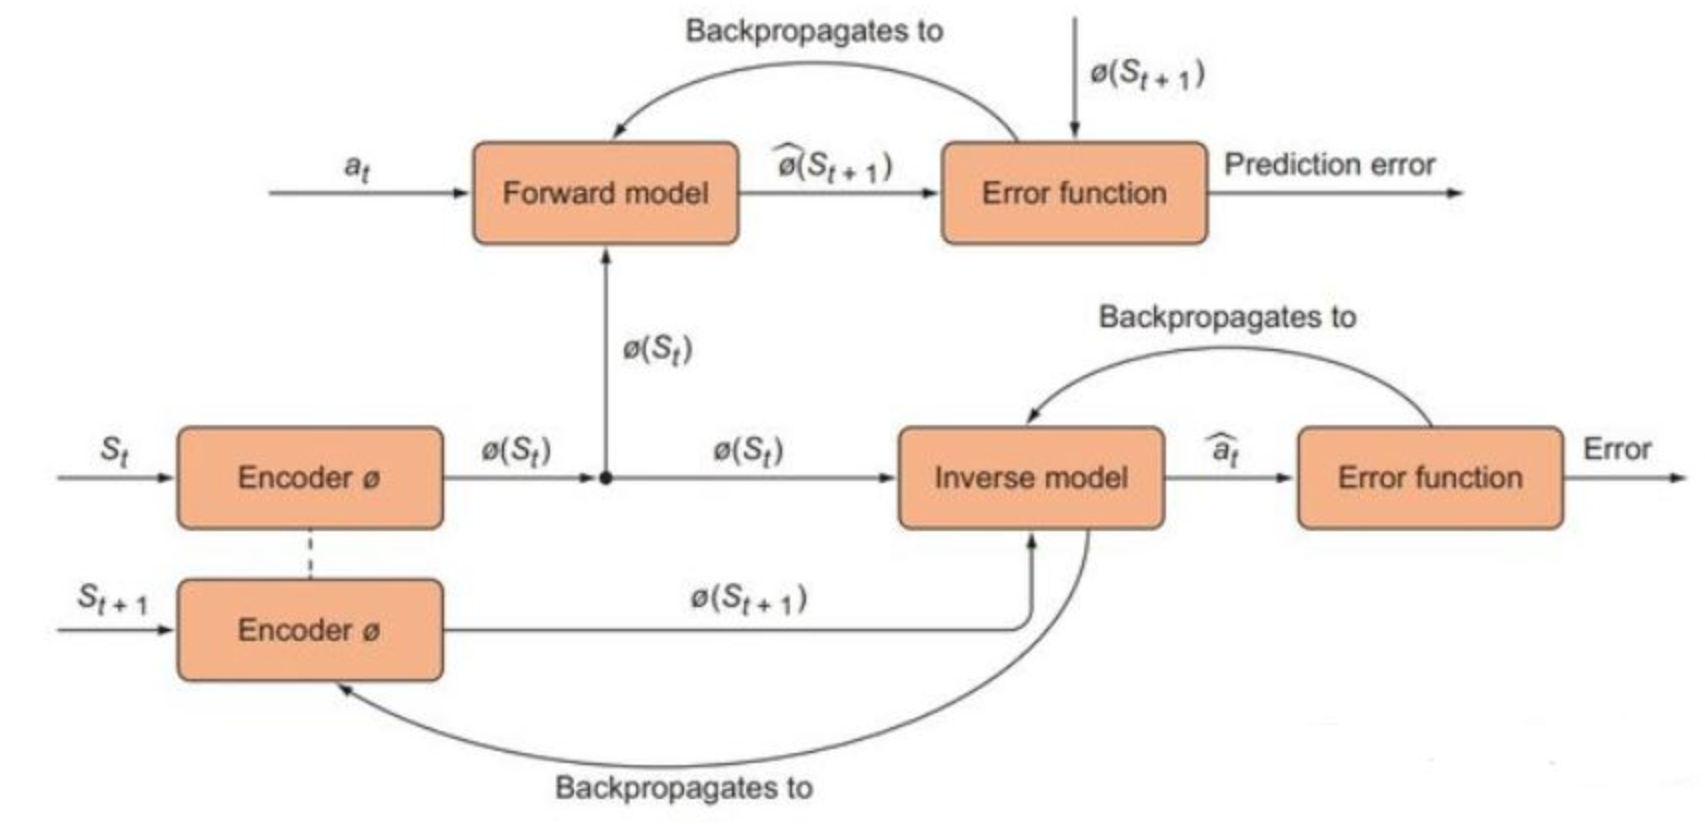
\includegraphics[width=0.5\linewidth]{figure/BackPropagation.png}
	\caption{The back propagation of ICM.}
	\label{fig:enter-label}
\end{figure}


\subsection{Dropout for exploration}
This method aims to enhance the exploration ability of reinforcement learning (RL) agents by introducing dropout into the neural network architecture. For the actor-critic structure algorithm, dropout is mainly added to the fully connected layer of the action to achieve exploration of the action space.


\section{Implementation details}
\subsection{Observation space and stating state}
The car racing environment consists frames of game state, where each frame is a $96\times 96\ RGB$ image of the car and race track, represented as $Box(0,255,(96,96,3),uint8)$ in Gymnasium package.

\subsection{Action space}
We utilize the continuous action space: steering ($-1$ is full left and $+1$ is full right), gas and brake, representing as $Box([-1,0,0],1.0,(3,),float32)$, as 3-dimensional array where action[0] is the steering direction, action[1] is gas pedal and action[2] is brake pedal.

\subsection{Extrinsic Reward setting}
The agent will receive reward -1 every frame and +1000/N
for every track tile visited, where N is the total number of tiles
visited in the track. If the car out of the edge of the environment then give -100 reward. The goal is to finish the race successfully in the least number of frames possible (fast). 

\section{Experiment}

\section{Conclusion}
TODO
\section{Others}

\bibliographystyle{IEEEtran}
\bibliography{IEEEabrv,reference}

\end{document}
